\chapter{Appendix to Chapter~\ref{ch:atrds}}
\label{app:atrds}

Code for the \href{https://github.com/jz268/atm_generative}{data} and \href{http://github.com/jz268/BayesAirATRDS2025}{inference} components provided on github at their respective links.

\section{Gradient Boosted Tree Regression}

As an initial step before we developed the method in \cref{ch:atrds}, we first attempted to reproduce the results of previous studies that used gradient boosted trees to directly regress on flight data from individual flights, with associated meteorological conditions at the corresponding time \cite{WU2022100030} One finding was that departure delay was a significant factor, which makes sense because if a flight leaves its origin late, it will also arrive at its destination late unless it tries to make up some time along its route, which may not always be possible.

After cleaning, processing, and merging the schedule and weather data for flights between Los Angeles International Airport (LAX) and John F. Kennedy International Airport (JFK), we found similar results using the XGBoost library \cite{Chen:2016:XST:2939672.2939785}. \cref{fig:importance-arr-dep} shows feature importance, based on the default ``number of times a feature is used to split the data across all trees'', when the target variable is set to either arrival or departure delay. Here, ``DepTimeMinutes'' refers to departure time, and ``CRSDepTimeMinutes'' refers to scheduled departure time. Both times are in minutes past midnight. As expected, we see that the most significant feature is departure time in both cases.

\begin{figure}
    \centering
    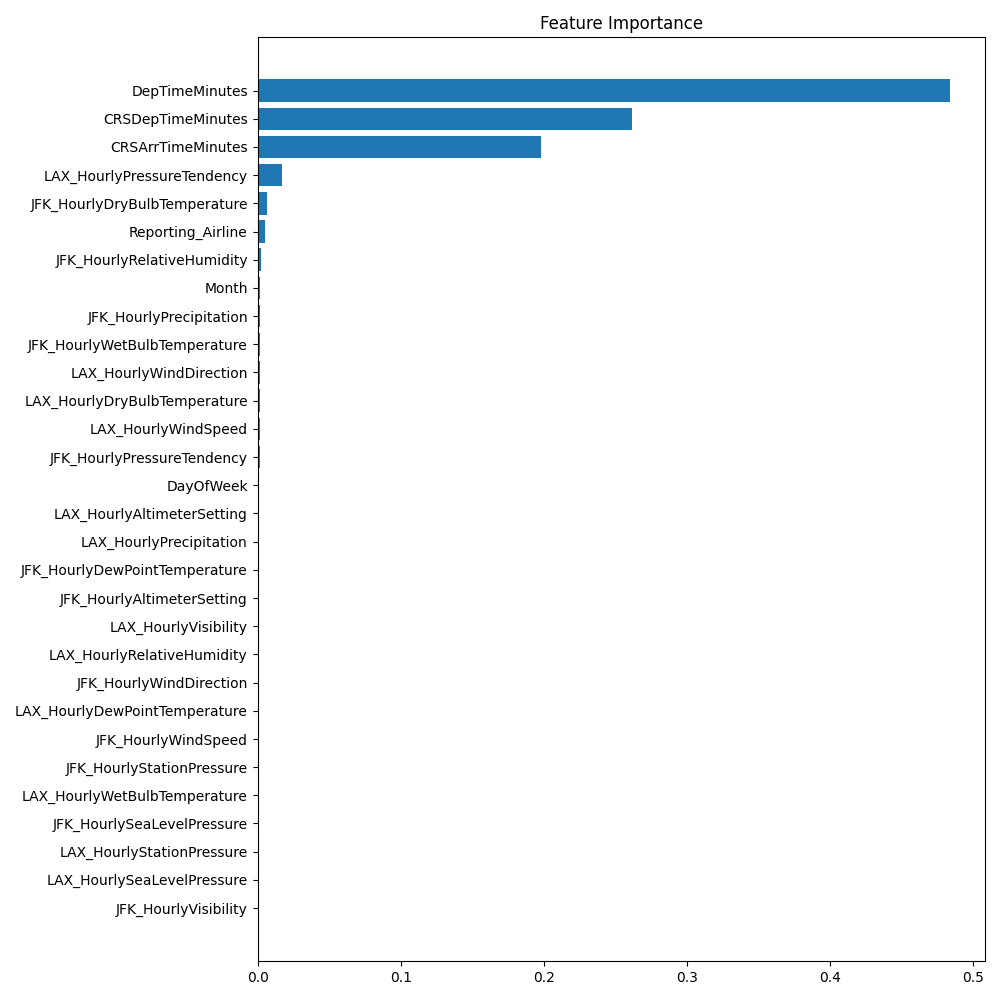
\includegraphics[width=0.49\linewidth]{media/features_ArrDelay.png}
    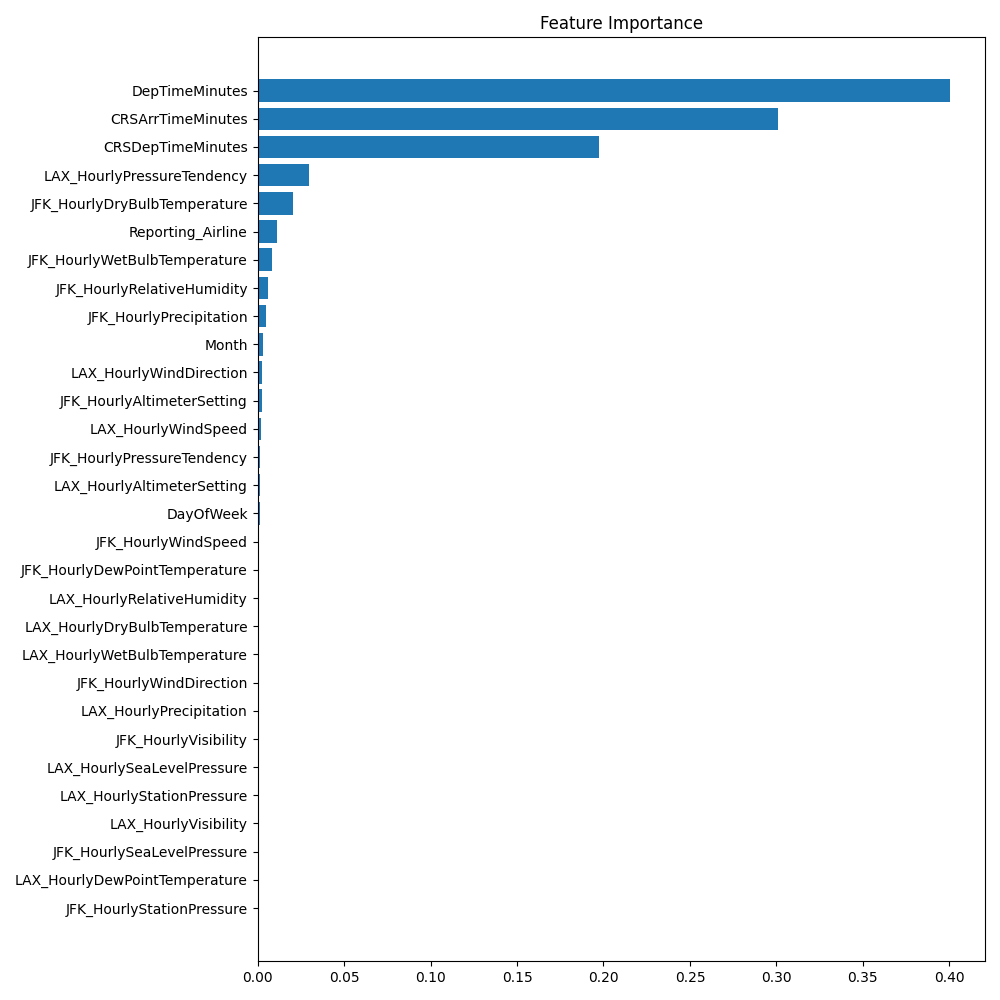
\includegraphics[width=0.49\linewidth]{media/features_DepDelay.png}
    \caption{Feature importance when target is arrival (left) and departure (right) delays.}
    \label{fig:importance-arr-dep}
\end{figure}

\begin{figure}
    \centering
    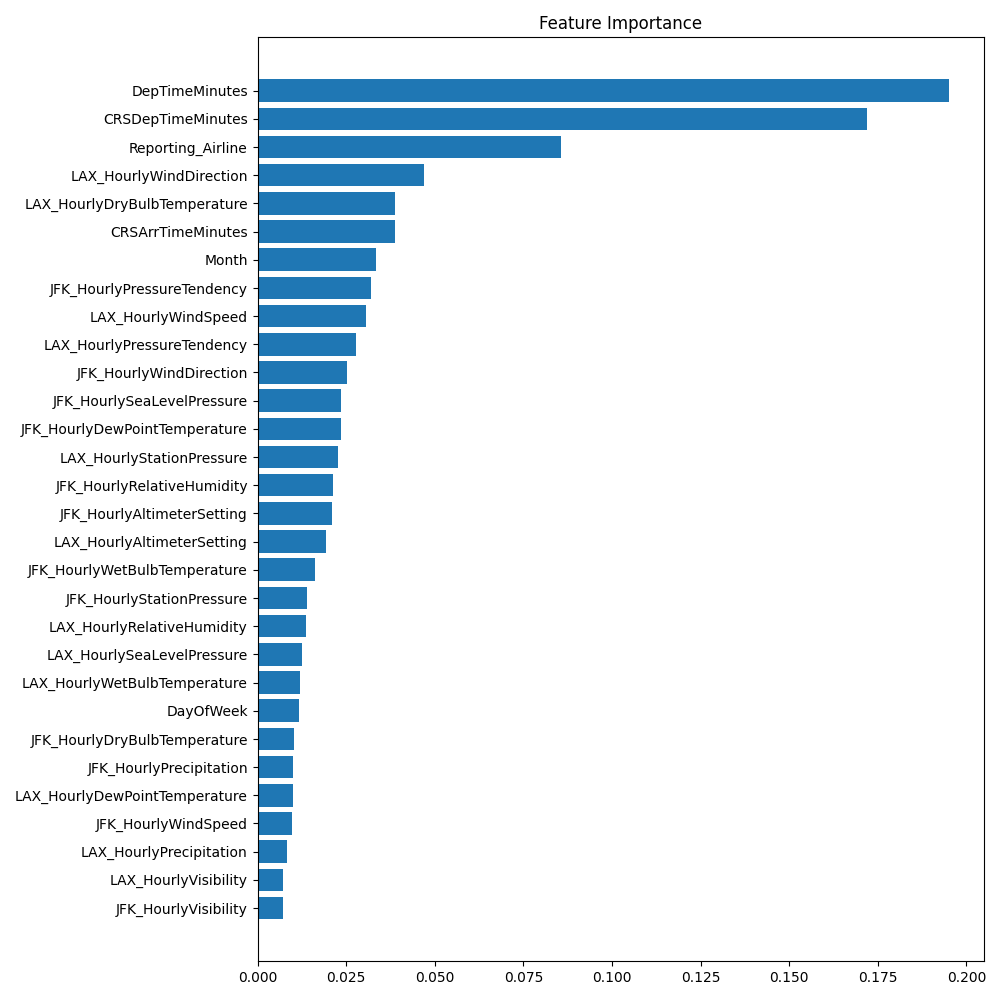
\includegraphics[width=0.49\linewidth]{media/features_NASDelay.png}
    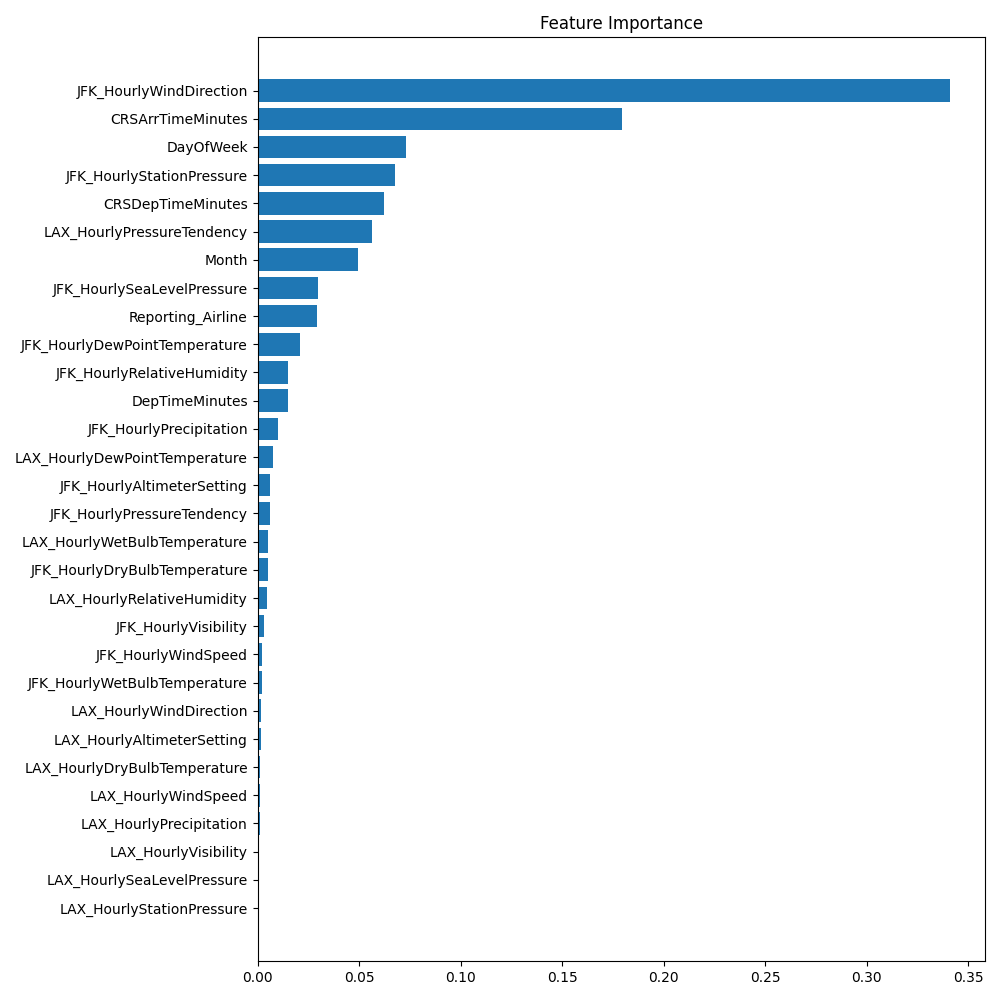
\includegraphics[width=0.49\linewidth]{media/features_WeatherDelay.png}
    \caption{Feature importance when target is NAS (left) and weather (right) delays.}
    \label{fig:importance-nas-weather}
\end{figure}

For NAS and weather delays in \cref{fig:importance-nas-weather}, we also see similar results, but they are slightly different. This is probably because there was not actually that much data with an NAS delay or weather delay actually reported, in comparison to the usual arrival and departure delays. We also tried to isolate the accumulated delay at a particular airport, which we called ``NewDelay'', from subtracting the departure delay from the arrival delay of a flight. Feature importance is shown in \cref{fig:importance-new}. We can see that we do not have any useful results anymore. This suggests that working with flights individually is not enough, and that we need to include the temporal structure somehow, for example, by working with entire days at a time similarly to the LGA case study.

\begin{figure}[hb]
    \centering
    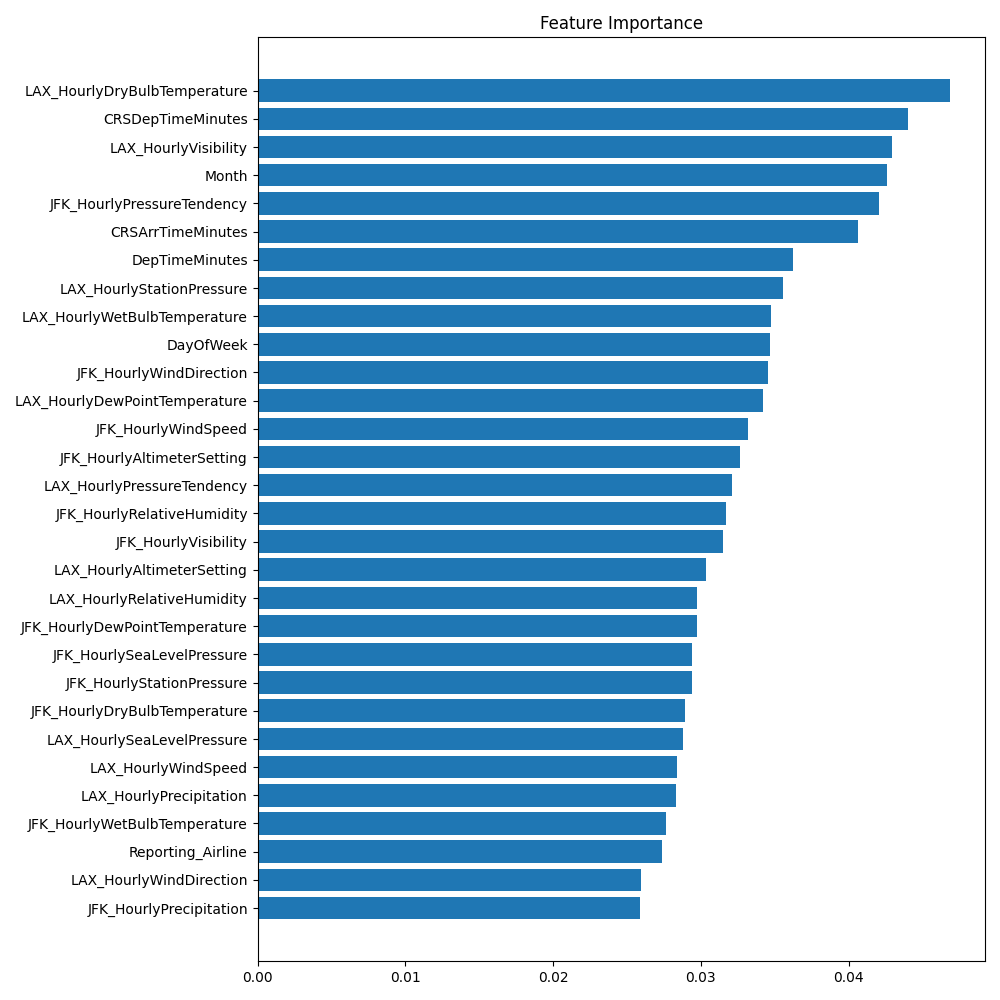
\includegraphics[width=0.75\linewidth]{media/features_NewDelay.png}
    \caption{Feature importance when target is new delays, i.e. arrival minus departure.}
    \label{fig:importance-new}
\end{figure}

\section{Aircraft Flows at LGA}

\begin{figure}[ht]
    \centering
    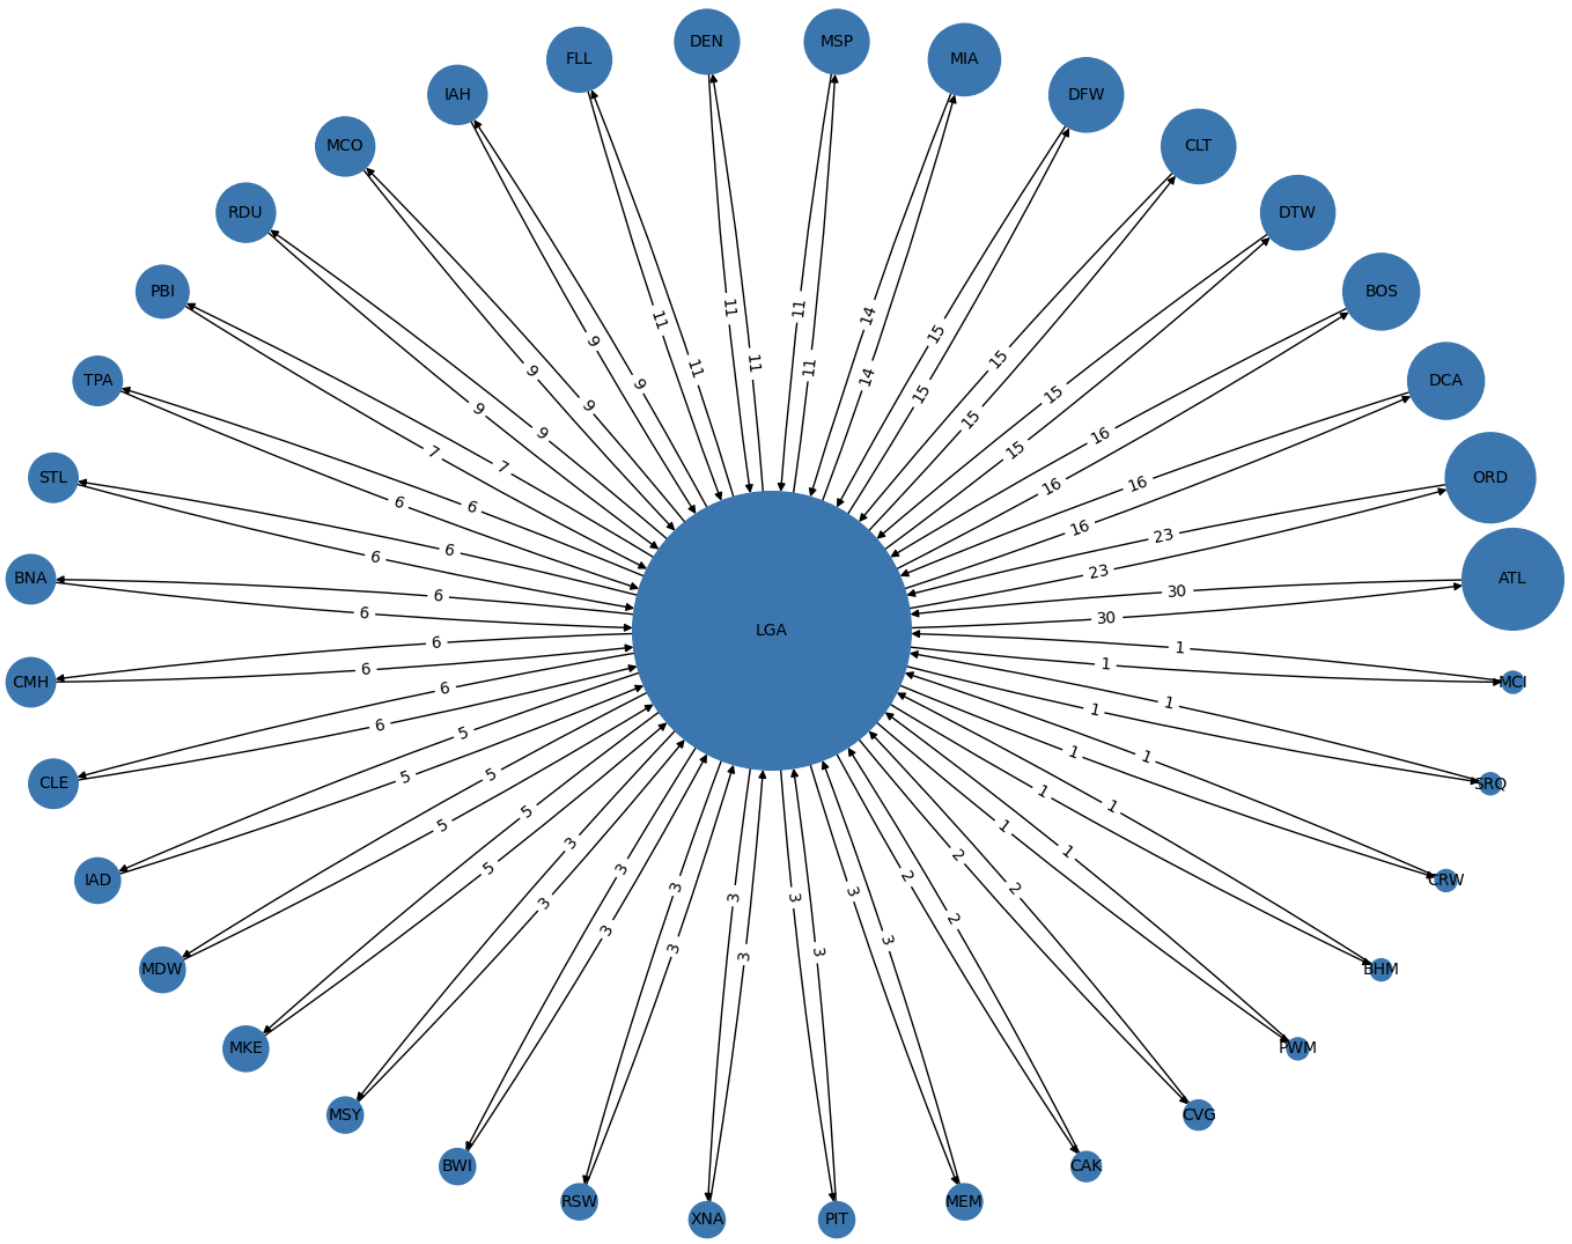
\includegraphics[width=\linewidth]{media/lga_reduced_2012_12_12_clean_cropped.png}
    \caption{Counts of both incoming and outgoing flights between LaGuardia Airport and each of its neighbors on 2012-12-12. Larger node size also indicates more flights.}
    \label{fig:lga-flows-diagram}
\end{figure}

\cref{fig:lga-flows-diagram} shows an example day of flights for LGA, represented as a directed network where the weight placed on each edge is the number of flights going in that direction. We can see that flights are scheduled to have the same number going each way, which makes sense because it is desirable for stability to have fleet levels and reserves at a particular node to stay relatively constant over time.

\section{Cascading Cancellations}

One possible direction for improving the simulation would be to more carefully track the likely dependency structure of flights throughout the day, using the schedule. This came up when analyzing days with many cancellations. For some routes, it seemed like the same aircraft was supposed to be used in sequence, but at some point, one flight was canceled, or delayed for a long time due to diversion, and all subsequent flights were then canceled. With a single airport, it is not as complicated, especially since many flights seemed to mainly be going back and forth between two nodes. However, the network case is likely more complicated, especially since different airlines may schedule their fleet differently.